\documentclass[a4paper,12pt]{report}

\usepackage{alltt, fancyvrb, url}
\usepackage{graphicx}
\usepackage[utf8]{inputenc}
\usepackage{float}
\usepackage{xcolor}
\usepackage{hyperref}

% Questo commentalo se vuoi scrivere in inglese.
\usepackage[italian]{babel}

\usepackage[italian]{cleveref}

\title{Relazione per\\``Programmazione ad Oggetti''}

\author{Simone Alocchi\\simone.alocchi@studio.unibo.it
\\Enrico Ancarani\\enrico.ancarani@studio.unibo.it
\\Stefano Baiano\\stefano.baiano@studio.unibo.it
\\Andrea Monti\\andrea.monti24@studio.unibo.it}
\date{\today}


\begin{document}

\maketitle

\tableofcontents

\chapter{Analisi}

\section{Descrizione e requisiti}

Il software ha come obiettivo di creare una copia del gioco da tavolo "Il Labirinto Magico" della Ravensburger.
%
L'intento principale è di riprodurre le dinamiche e le meccaniche del gioco
 originali, ma con l'aggiunta di elementi nuovi come per esempio i 
powerUps e un nemico che si muove all'interno del labirinto.
%
Il gioco si sviluppa su un'idea di competizione diretta tra i giocatori,
 configurandosi quindi come un'esperienza di tipo "tutti contro tutti".

\subsection*{Requisiti funzionali}
\begin{itemize}
	\item L’utente può avviare una partita scegliendo da 2 a 4 giocatori.
	%
	In base al numero di giocatori selezionati, varieranno le dimensioni del labirinto e la gestione dei turni.
	%
	Tutti i giocatori devono essere controllati manualmente, quindi si consiglia di giocare insieme ad amici.
	\item Il labirinto deve essere generato con una dimensione fissa che varia in base al numero di giocatori presenti.
	%
	Questa scelta riguarda esclusivamente la fase iniziale della partita: il labirinto potrà poi essere modificato durante il gioco.
	\item Il gioco permette di modificare il labirinto inserendo la tessera rimasta fuori dalla generazione iniziale.
	%
	Inserendo la tessera da uno dei lati del labirinto, tutte le tessere nella riga o colonna corrispondente si spostano di una posizione.
	%
	La tessera che esce dal lato opposto diventa la nuova tessera disponibile per la modifica al turno successivo.
	\item All'interno del labirinto vengono generati degli obiettivi che i giocatori possono raccogliere.
	\item Ogni volta che un giocatore raccoglie un obiettivo, riceve un power-up a utilizzo singolo.
	\item In ogni momento, l’interfaccia grafica mostra una classifica aggiornata con i nomi dei giocatori e i loro punteggi attuali.
	\item L'utente può decidere di giocare con all'interno del labirinto un nemico con movimento casuale.
	\item L’interfaccia grafica si aggiorna automaticamente dopo ogni azione compiuta.
\end{itemize}

\subsection*{Requisiti non funzionali}
\begin{itemize}
	\item Creare un nemico intelligente che se possibile insegue il giocatore.
	\item Salvataggio e caricamento di una partita giocata in precedenza e non finita.
\end{itemize}

\section{Modello del Dominio}

Il sistema rappresenta un gioco da tavolo digitale ambientato in un labirinto dinamico. Il labirinto viene generato con tessere posizionate casualmente. 
I giocatori partono dagli angoli della mappa, mentre un nemico viene inizialmente posizionato al centro. 
Gli obiettivi da raccogliere sono distribuiti in tessere casuali all'interno del labirinto.
Ogni volta che un turno inizia si eseguono 3 fasi in questa sequenza:
\begin{itemize}
	\item Fase di modifica: Il giocatore inserisce la tessera esterna in uno dei lati del labirinto ruotata a suo piacimento, facendo slittare la riga o la colonna corrispondente. Questo cambia dinamicamente la forma del labirinto.
	\item Fase del Giocatore: Il giocatore può:
	\begin{itemize}
		\item Muoversi all’interno del labirinto senza limiti di passi, in base alle connessioni disponibili tra le tessere.
		\item Usare un eventuale power-up ottenuto precedentemente.
	\end{itemize}
	\item Fase del Nemico: Il nemico si muove secondo una logica definita e se entra in contatto con un giocatore, gli rimuove un obiettivo raccolto e lo riposiziona nel labirinto.
\end{itemize}
Durante la partita, i giocatori devono cercare di raccogliere il maggior numero possibile di obiettivi. Ogni obiettivo raccolto fornisce al giocatore un power-up utilizzabile una sola volta.
Al termine del gioco (quando tutti gli obiettivi sono stati raccolti), vince il giocatore che ne ha ottenuti di più.
In caso di parità, viene generato un ulteriore obiettivo per determinare il vincitore continuando la partita.

\begin{figure}[H]
	\centering{}
	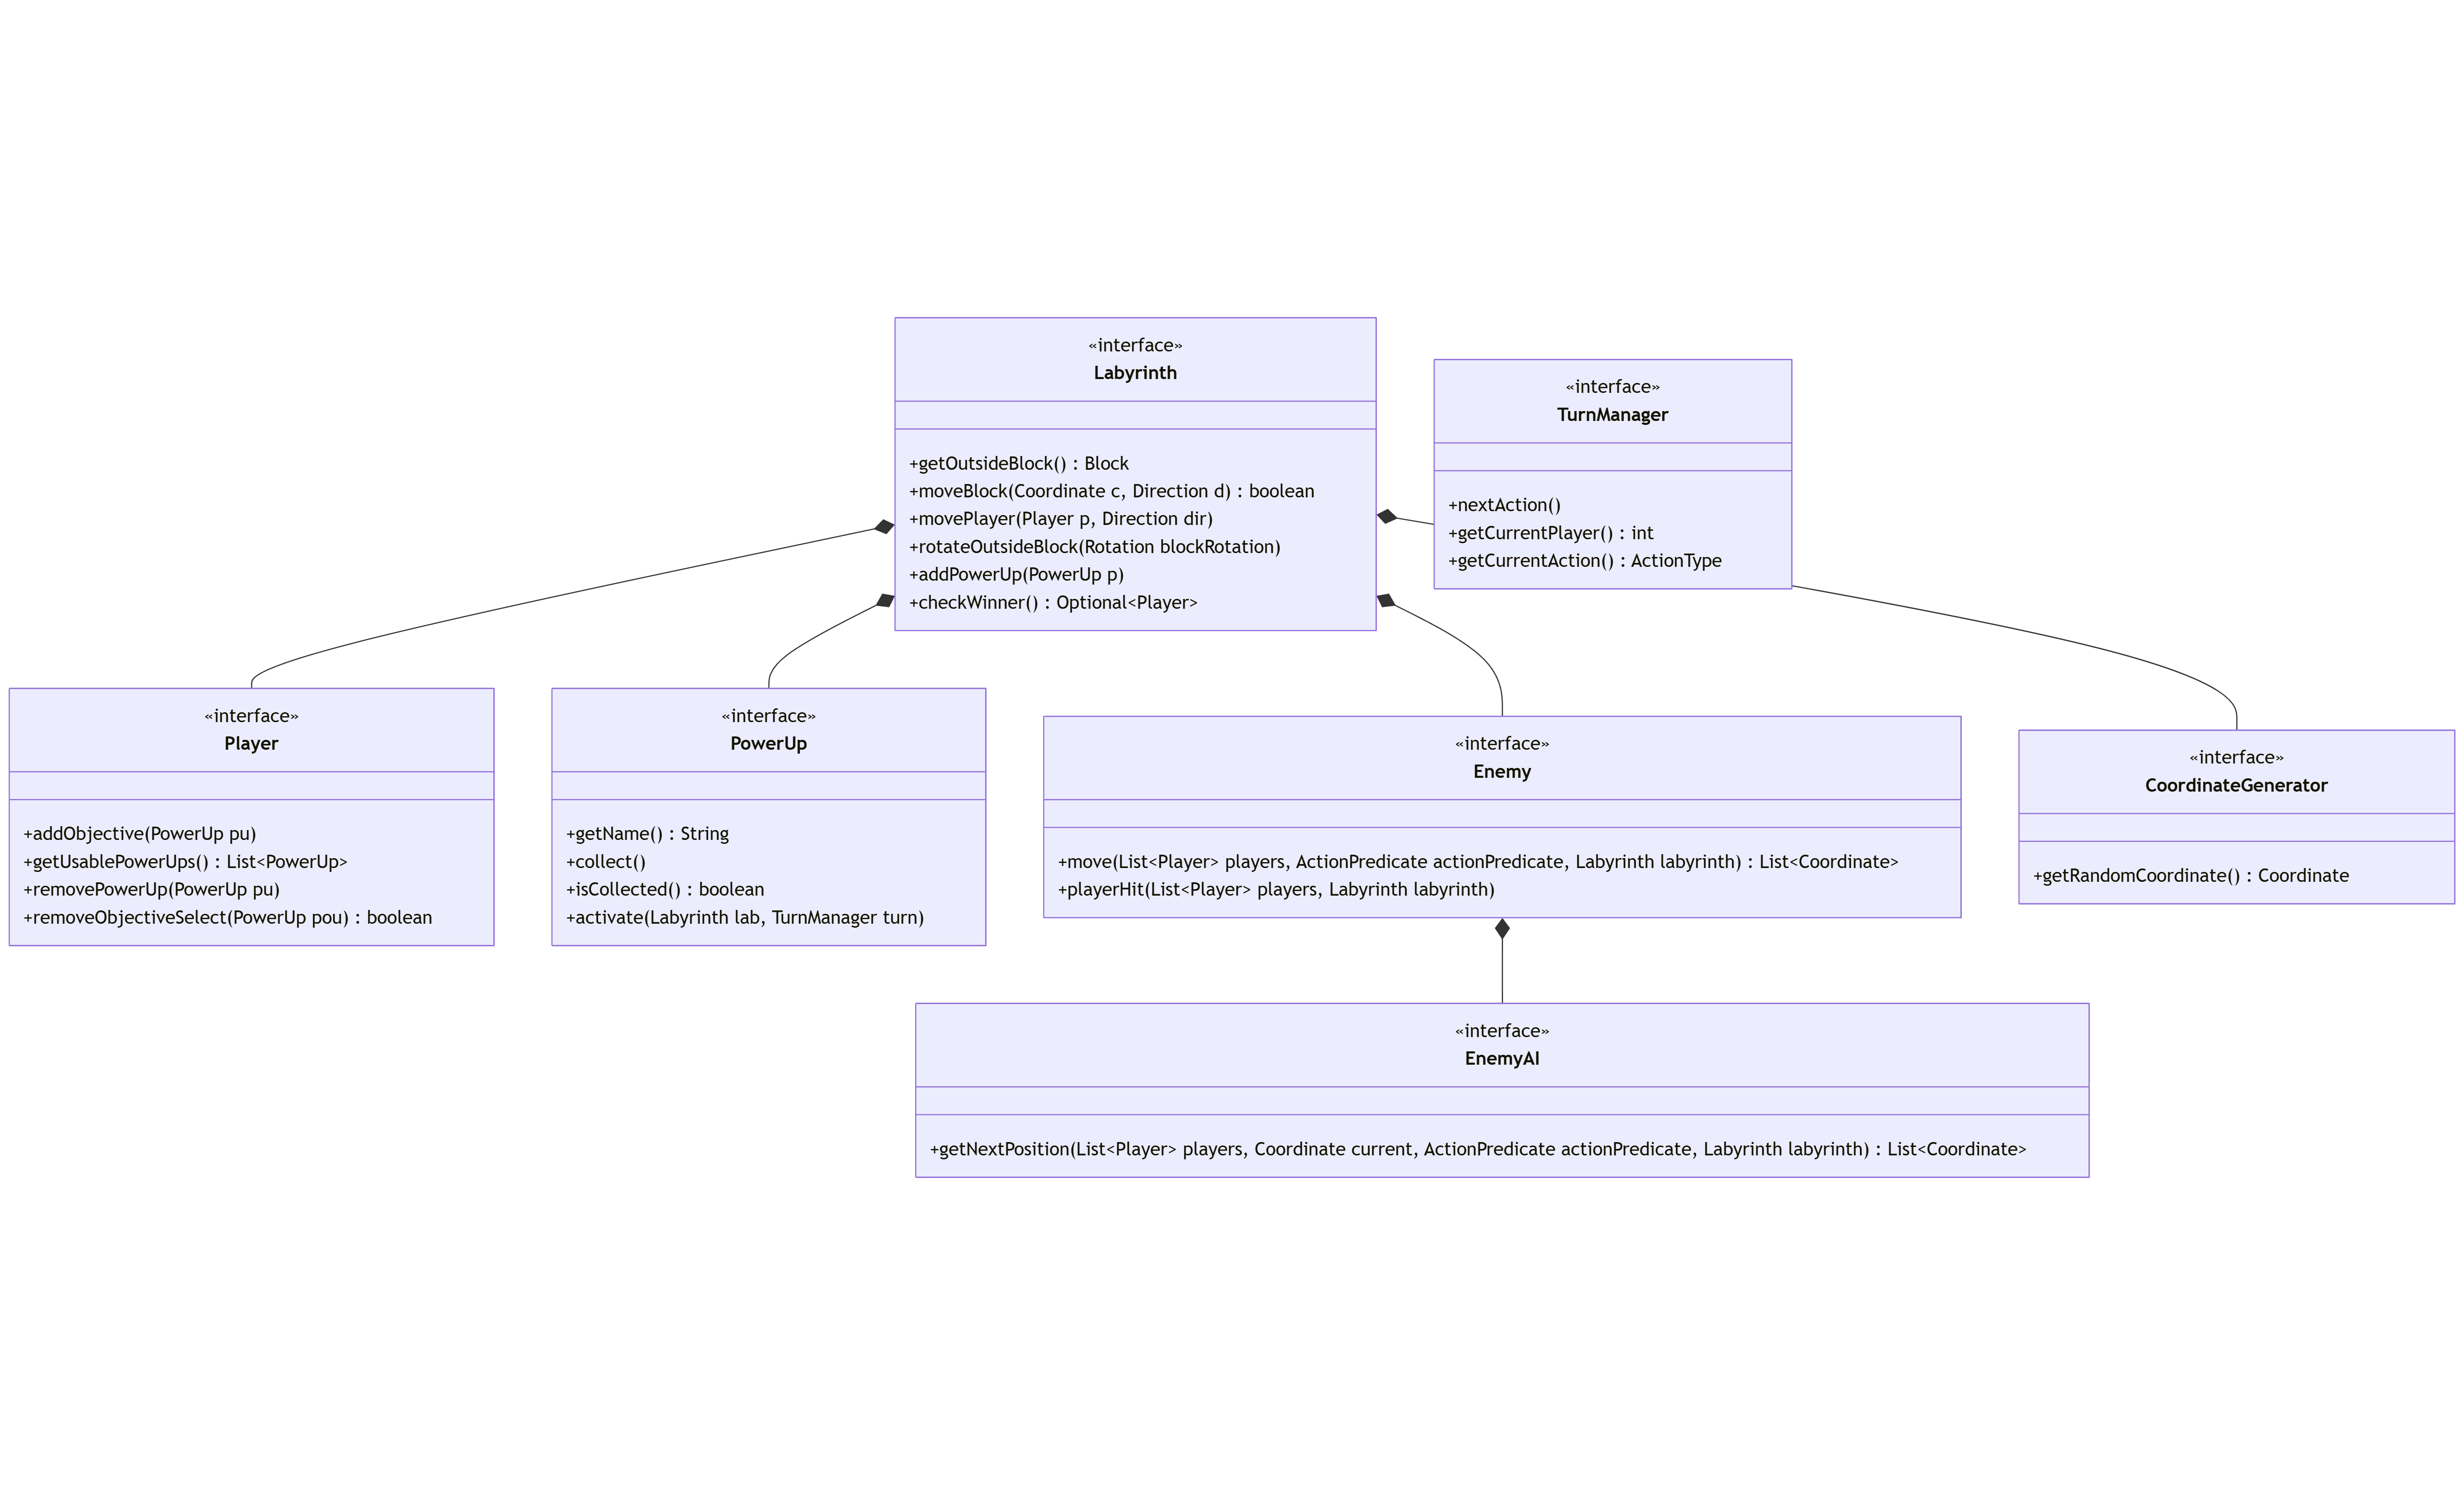
\includegraphics[width=14cm]{img/DominioElementi.png}
	\caption{Schema UML del dominio per la parte degli elementi}
	\label{img:dominio elementi}
\end{figure}

\begin{figure}[H]
	\centering{}
	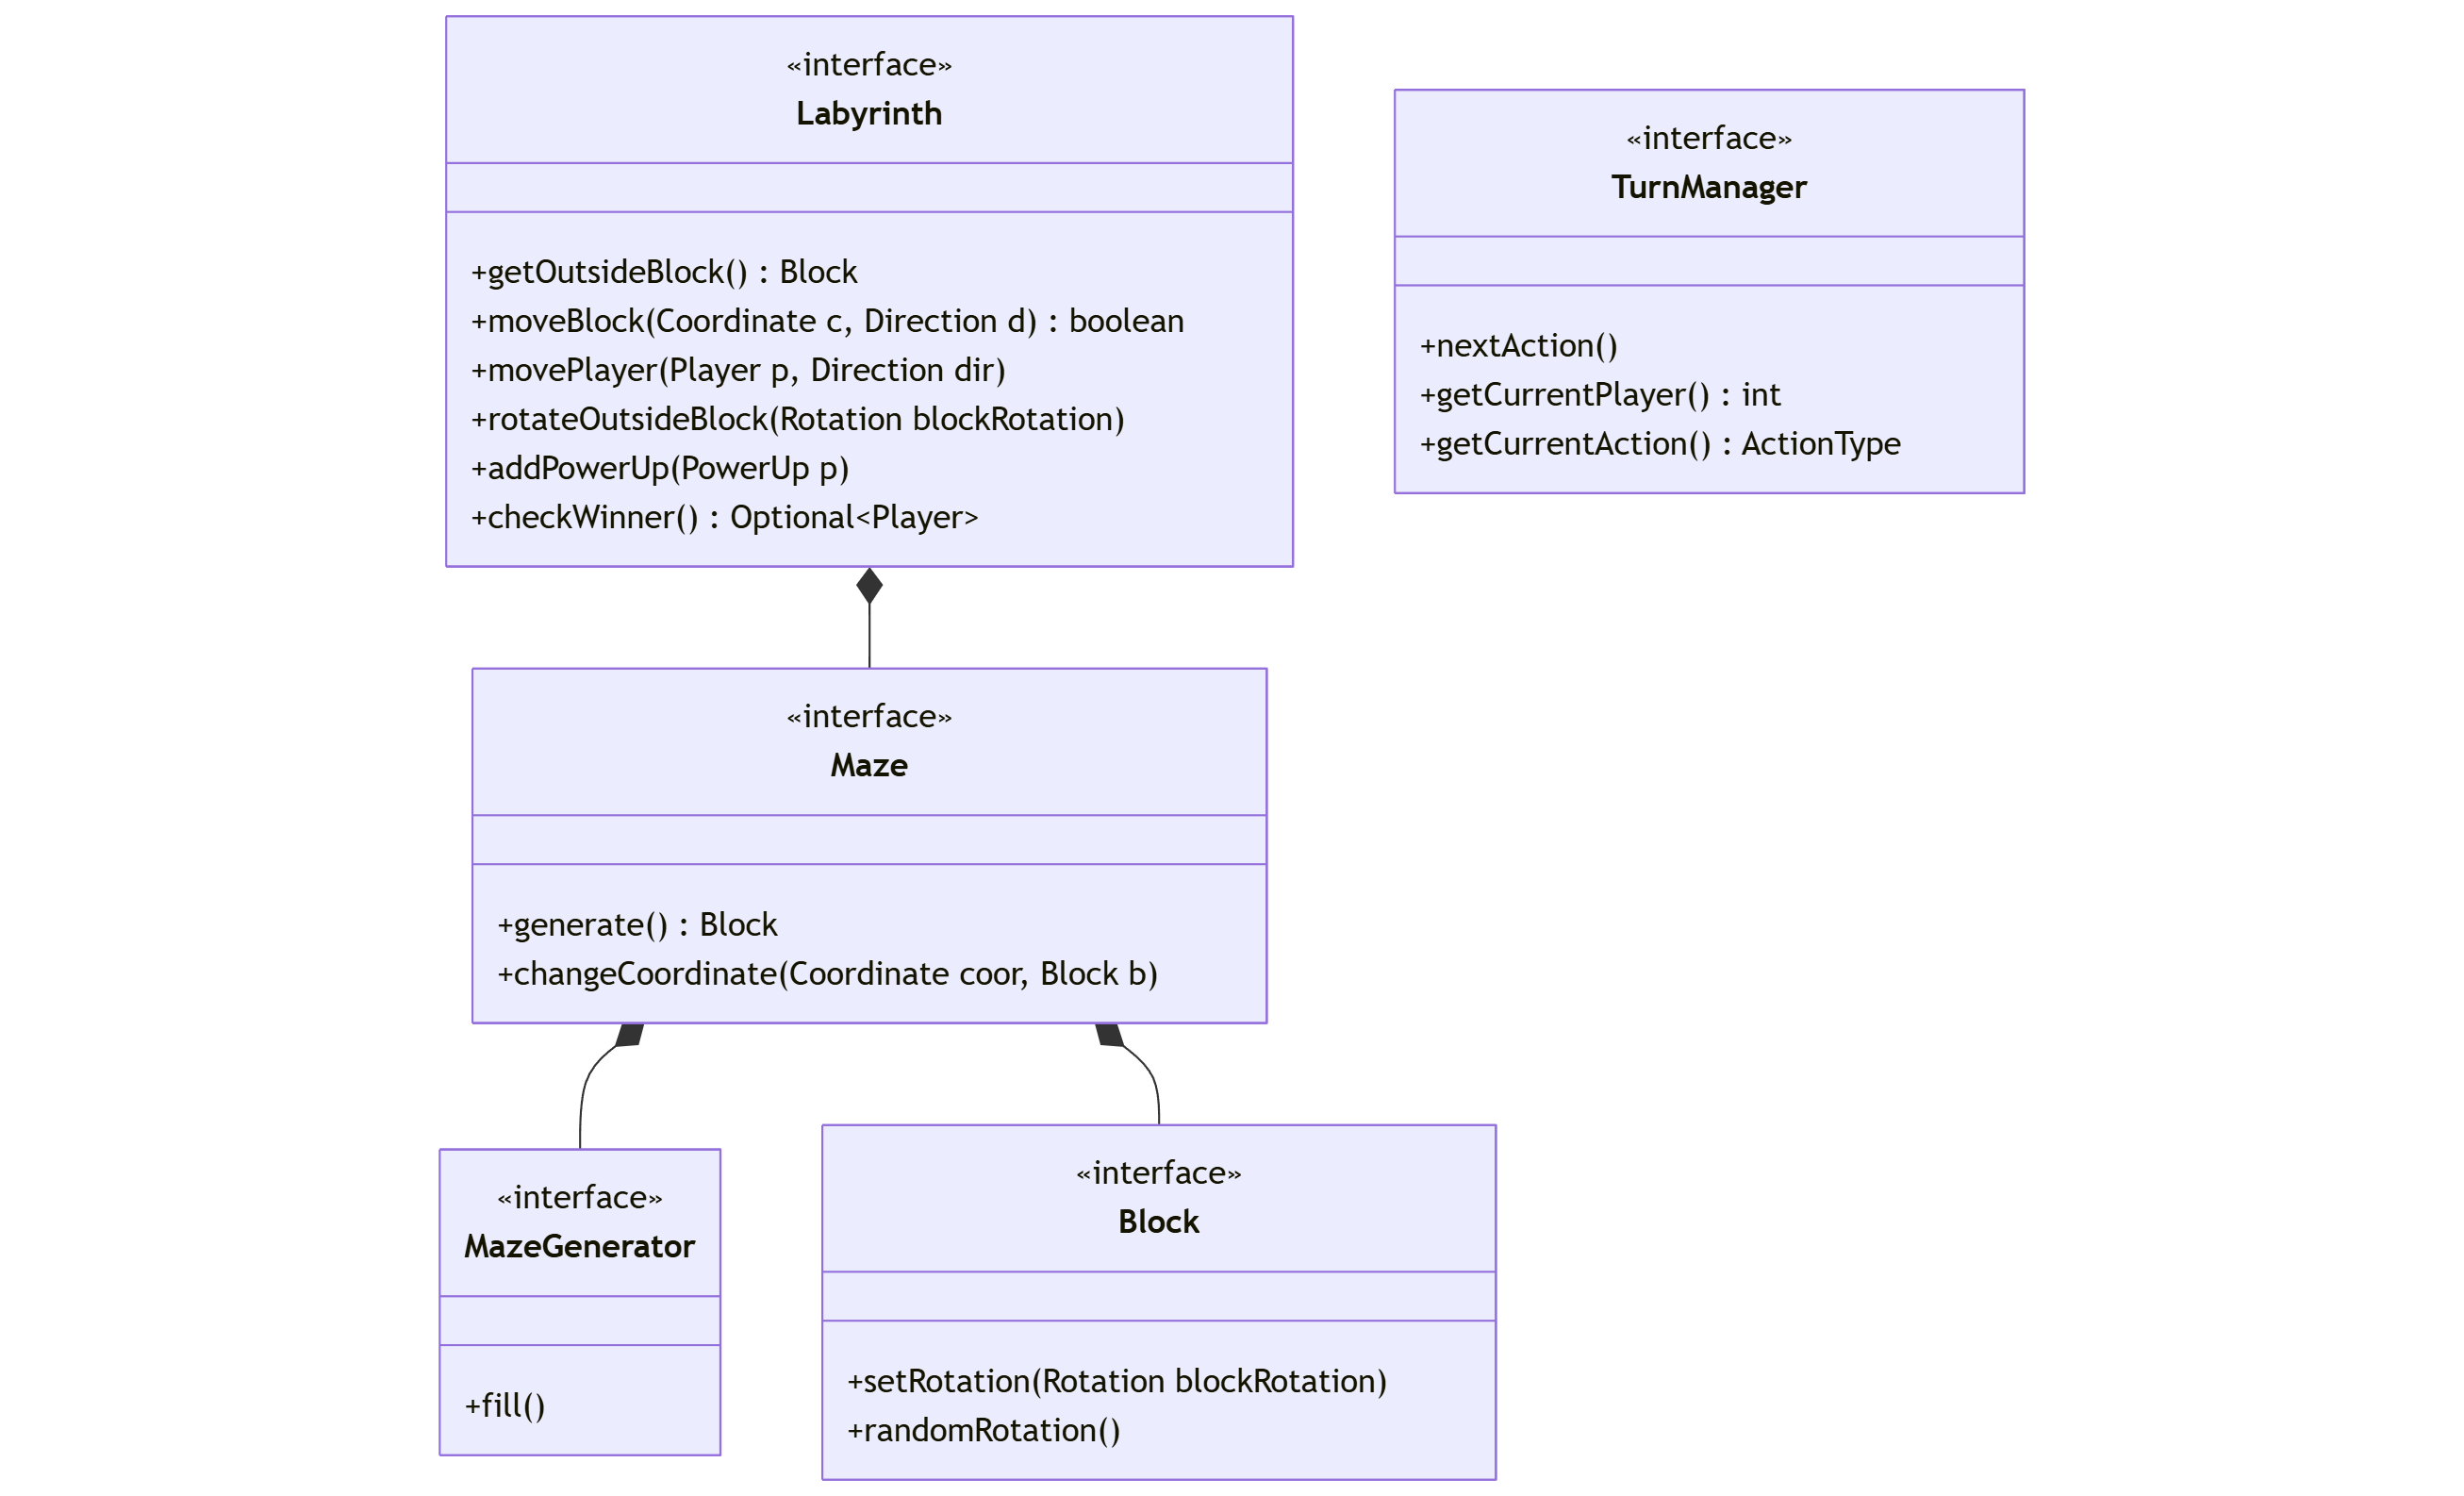
\includegraphics[width=14cm]{img/DominioLabirinto.png}
	\caption{Schema UML del dominio per la parte del labirinto}
	\label{img:dominio labirinto}
\end{figure}

\chapter{Design}

\section{Architettura}
Il progetto è strutturato secondo il pattern architetturale MVC (Model-View-Controller). 
Il punto di partenza dell’interazione fra utente e software inizia con la view MainMenu, la quale offre diverse opzioni:
\begin{itemize}
	\item Avviare una nuova partita.
	\item Caricare una partita salvata.
	\item Accedere alle impostazioni di gioco.
	\item Uscire dall’applicazione.
\end{itemize}
La parte logica del MainMenu viene affidata ad un MainMenuController, 
il quale compie operazioni con la view SettingsMenu ed il LoadController, che serviranno a gestire l’avvio della partita e il cambiamento delle impostazioni di gioco.
Se si seleziona di accedere alle impostazioni di gioco verrà mostrata la view SettingsMenu che permette all’utente di configurare i parametri di gioco, quali:
\begin{itemize}
	\item Difficoltà del nemico.
	\item Numero di giocatori.
	\item Numero di power-up/obiettivi disponibili.
	\item Se il nemico è presente.
\end{itemize}
Il settingsController, come nel caso del MainMenuController, si occupa delle operazioni logiche, 
quali il salvataggio delle impostazioni appena scelte dall’utente tramite la classe  SaveController, in grado di scrivere su file.
In caso di avviamento o di caricamento della partita precedente il MainMenuController richiamerà alcune funzioni del 
LoadController, che raccoglieranno a seconda del caso i dati dei settings oppure la partita precedente, attraverso i file di salvataggio.
All’avviamento della partita viene creato un GameController che genererà tutti gli elementi del gioco tramite una classe Builder, 
e li assegnerà alle classi sottostanti. Inoltre, il GameController si occuperà della coordinazione delle componenti principali quali:
\begin{itemize}
	\item Labyrinth, che rappresenta l’ambiente di gioco con tutti i suoi elementi.
	\item TurnManager, responsabile della gestione dei turni tra i giocatori.
	\item ActionController, gestore delle azioni e delle loro conseguenze.
	\item SaveController, per il salvataggio automatico dello stato di gioco.
\end{itemize}
A seguito viene creata la view principale del gioco, la GameView, responsabile dell’interfaccia tra utente ed il gioco. Questa si occupa di:
\begin{itemize}
	\item Creare gli elementi dell’interfaccia (pulsanti, label, ecc.).
	\item Aggiornare i componenti grafici in base ai cambiamenti nel model.
	\item Visualizzare lo stato corrente del gioco (punteggi, turno corrente, ecc.).
	\item Permettere l’interazione dell’utente con i suoi elementi.
\end{itemize}
Le operazioni logiche, anche in questo caso, sono delegate ad un’altra classe, la LogicGameView, che funge da intermediario tra GameView e GameController, 
offrendo metodi per ottenere informazioni sullo stato del gioco e per eseguire azioni in risposta agli input dell’utente.
Questi input utente vengono elaborati dall’ActionController, che determina il tipo di azione da eseguire e la applica al model. 
Prima di eseguire un’azione, consulta l’ActionPredicate, un componente di tipo ”semaforo” che stabilisce se un’azione è eseguibile 
in base alle condizioni attuali del model. Dopo ogni azione, la GameView si aggiorna.
\begin{figure}[H]
	\centering{}
	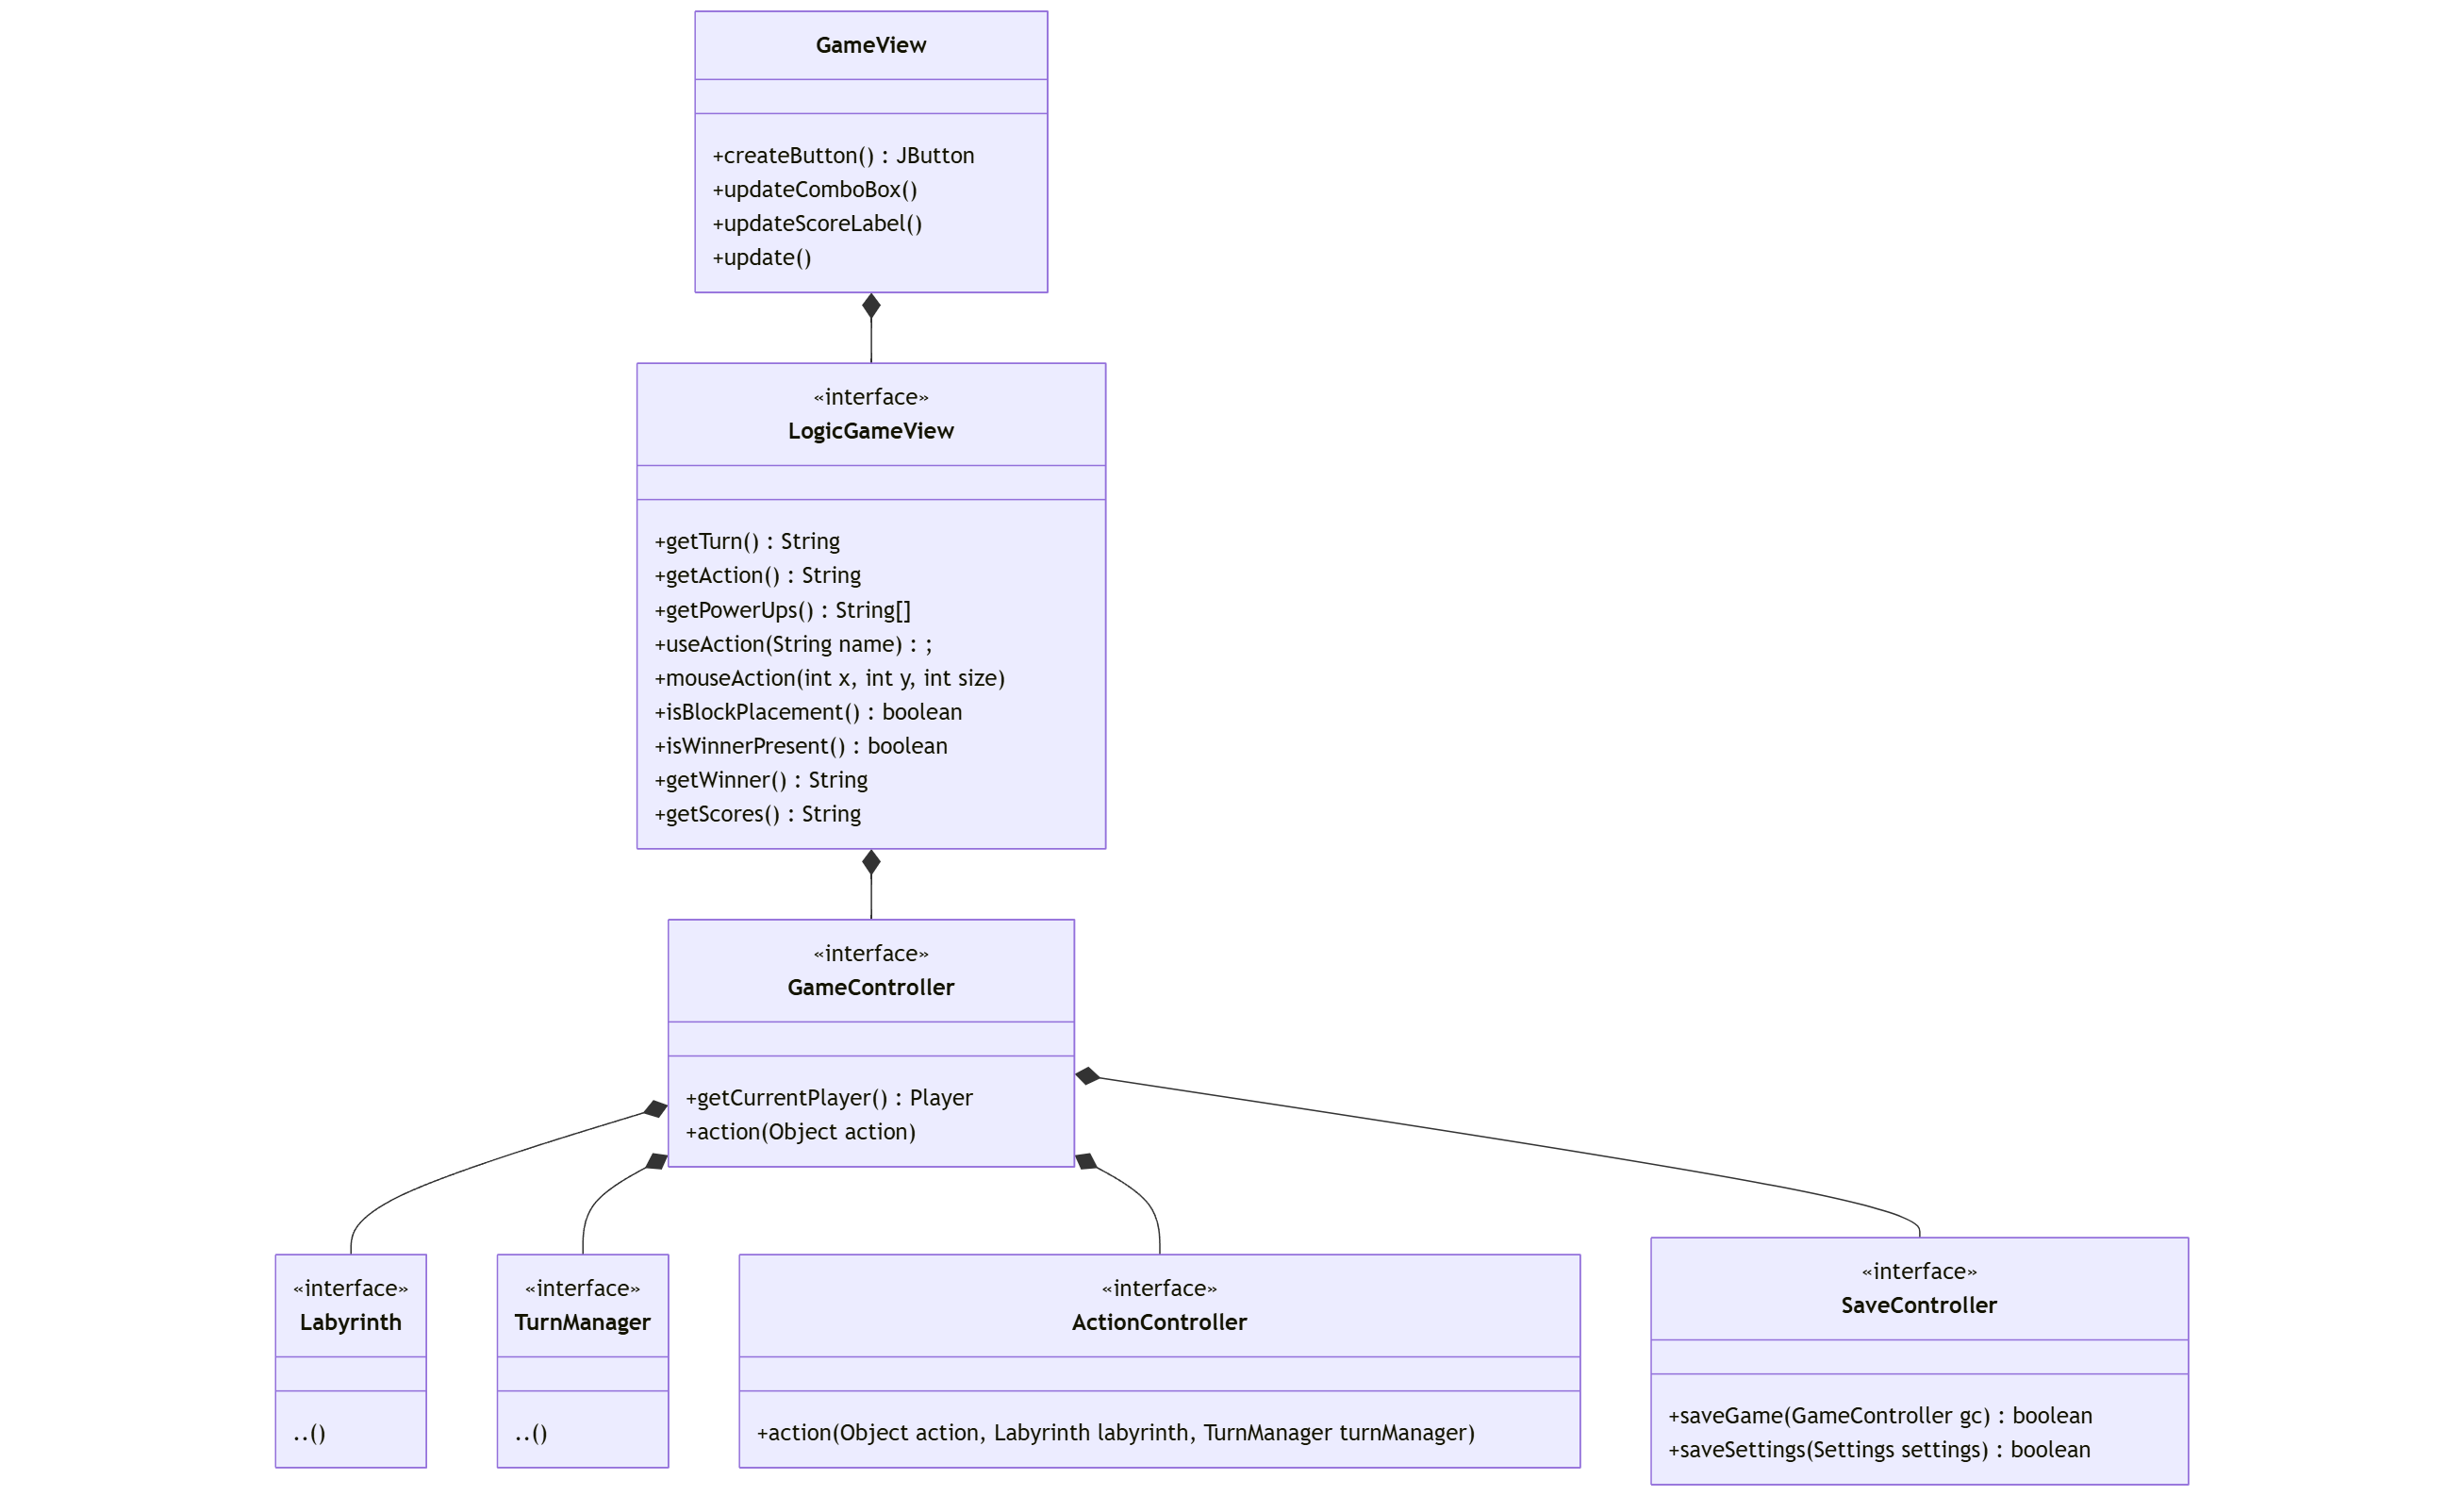
\includegraphics[width=14cm]{img/ArchitetturaGameView.png}
	\caption{Schema UML dell'architettura per la parte di gioco}
	\label{img:Architettura GameView}
\end{figure}

\section{Design dettagliato}

\subsection{Enrico Ancarani}
\textbf{Generazione del labirinto}
\\
\\
\textbf{PROBLEMA}\\
Nel gioco originale Labirinto Magico di Ravensburger, la composizione delle tessere è fissa: ci sono un numero predefinito di tessere a "L", a "T" e a linea retta, 
e la difficoltà e la giocabilità derivano dalla loro disposizione e rotazione. Tuttavia, il nostro gioco prevede la possibilità di cambiare le dimensioni del labirinto 
in base al numero di giocatori, rendendo impraticabile copiare esattamente il contenuto del gioco originale.
Inoltre, una generazione completamente casuale delle tessere rischia di rendere il labirinto poco giocabile: troppe tessere dello stesso tipo 
possono compromettere l’esperienza dell’utente.\\
\\
\textbf{SOLUZIONE}\\
Per risolvere questo problema, ho definito una gerarchia di classi orientata all’estensione e alla flessibilità.
\begin{itemize}
	\item \textbf{Maze}: è una classe astratta che definisce l’interfaccia e le funzionalità comuni di qualsiasi tipo di labirinto.
	\item \textbf{SimpleMaze}: è un’implementazione di Maze che utilizza la stessa composizione di tessere del gioco originale.
	\item \textbf{MazeGenerator}: è la classe responsabile della costruzione del labirinto: riceve in input un insieme predefinito di tessere 
	(fornite dalla sottoclasse di Maze), le posiziona sulla griglia assegnando a ognuna una coordinata e impendendo alla tessera di 
	essere riposizionata, e restituisce il labirinto completato con una tessera “extra” da usare per la meccanica di shift.
\end{itemize}
Durante la progettazione ho stabilito che le quattro posizioni di spawn dei giocatori (i quattro angoli del labirinto) 
devono contenere sempre tessere a “L” ruotate verso il centro, per garantire un inizio bilanciato e impedire generazioni scomode per i giocatori all'inizio. (labirinto di tessere angolo)
\\
\\
\textbf{PRO}
\begin{itemize}
	\item Facile estensione per diversi tipi di labirinti: Si possono creare estensioni di Maze che permettono in futuro all'utente di scegliere mappe di gioco con conformazioni 
	particolari.
	\item Chiarezza nella separazione di responsabilità: La gestione delle coordinate delle tessere viene fatta dal Maze, la generazione e assegnazione iniziale dal MazeGenerator e 
	la scelta di tessere dal SimpleMaze
	\item Template Method Pattern: viene utilizzato questo pattern per creare un ambiente facilmente estensibile e lasciare il comportamento generale del labirinto invariato.
\end{itemize}
\textbf{CONTRO}
\begin{itemize}
	\item È necessario implementare una nuova sottoclasse per ogni tipo di configurazione: ogni volta che si vuole un certo scenario con una scelta specifica di tessere bisogna 
	implementare una nuova sottoclasse di Maze
\end{itemize}
\begin{figure}[H]
	\centering{}
	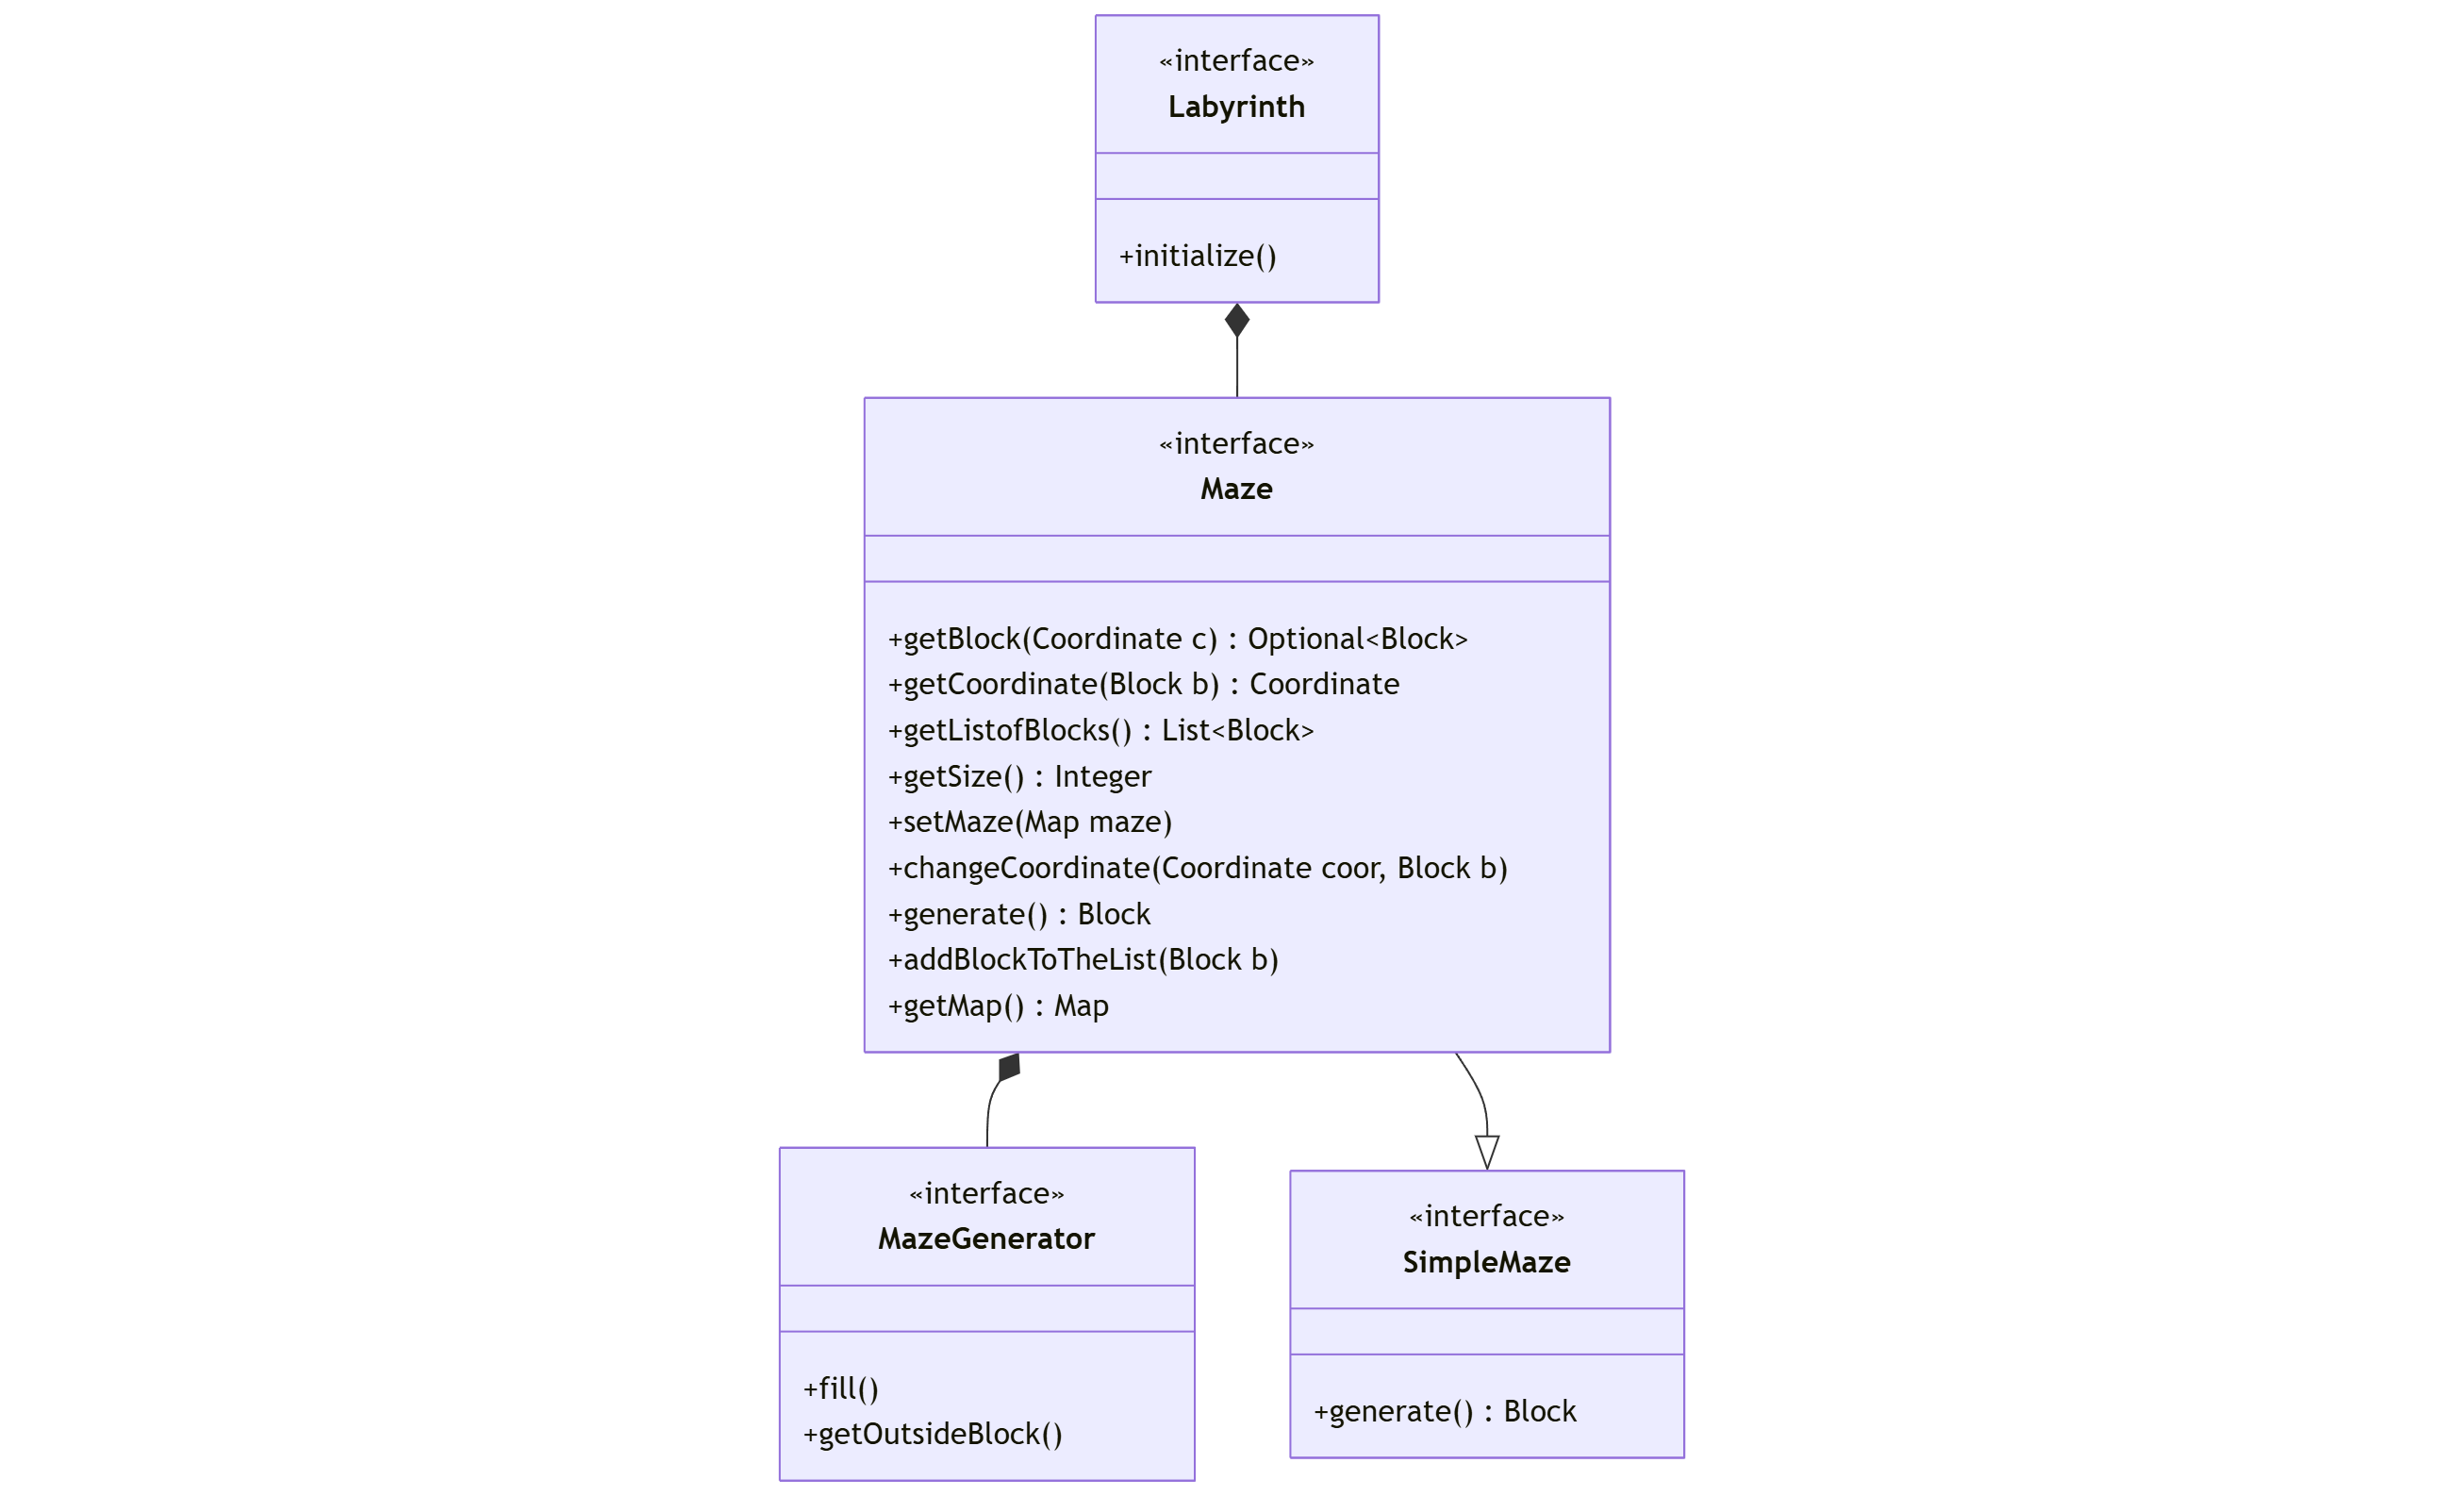
\includegraphics[width=14cm]{img/GenerazioneLabirinto.png}
	\caption{Schema UML della struttura per generare il labirinto}
	\label{img:Generazione Labirinto}
\end{figure}
\textbf{Gestione delle coordinate e coordinate iniziali}
\\
\\
\textbf{PROBLEMA}\\
Un aspetto centrale nello sviluppo del gioco è la gestione delle posizioni degli elementi sulla mappa.
Essa viene con diverse problematiche da risolvere:
\begin{itemize}
	\item Recupero della posizione: necessità di ottenere le coordinate a partire da un elemento e viceversa.
	\item Meccanica di shift: gestione dello spostamento delle tessere (e degli elementi sopra di esse) a seguito dell’inserimento della tessera extra.
	\item Effetto "Pac-Man": se un elemento viene spinto fuori dal labirinto, deve riapparire dalla parte opposta, mantenendo coerenza con la direzione dello spostamento.
\end{itemize}
\textbf{SOLUZIONE}\\
Una possibile soluzione iniziale era lasciare che ogni elemento conoscesse 
la propria posizione, ma questa scelta avrebbe complicato eccessivamente 
l’interazione tra elementi e labirinto. Pertanto, ho optato per un approccio centralizzato.
Per risolvere le problematiche sopra descritte, ho progettato la classe Labyrinth, 
responsabile della gestione centralizzata delle coordinate di tutti gli elementi del gioco: giocatori, nemico e powerup (obbiettivi).
Al suo interno la classe utilizza 2 componenti creati appositamente:
\begin{itemize}
	\item \textbf{DualMap}: struttura bidirezionale che collega elementi e coordinate, permettendo sia di trovare la posizione di un elemento, 
	sia di identificare cosa si trova in una determinata posizione.
	\item \textbf{CoordinateGenerator}: classe dedicata alla generazione delle coordinate iniziali, secondo logiche diverse in base al tipo di elemento.
\end{itemize}
La classe CoordinateGenerator è progettata per supportare la generazione delle coordinate in base alle seguenti esigenze:
\begin{itemize}
	\item PowerUp: la generazione avviene escludendo gli angoli del labirinto (riservati ai giocatori).
	\item Nemico: viene determinata la coordinata centrale del labirinto (calcolata sulla base della dimensione).
	\item Giocatori: la generazione avviene estraendo randomicamente i 4 angoli della mappa.
\end{itemize}
In ogni caso, le coordinate già estratte vengono rimosse dal set interno, garantendo unicità e prevenendo sovrapposizioni indesiderate.
Per quanto riguarda la meccanica di shift ho pensato che potesse bastare un metodo all'interno della classe Labyrinth.
Ho pensato che la responsabilità del metodo ricadesse proprio nel Labyrinth in quanto il metodo shift è alla base uno spostamento di coordinate.
Per funzionare al meglio ho deciso di suddividere i compiti del metodo su più metodi private in modo da permettere una chiara lettura e modifica.
Le funzioni suddivise sono: Determinare il tipo di shift (riga,colonna), calcolare la nuova posizione per ogni elemento, modificare la posizione delle tessere, modificare la posizione degli elementi,
controllare se la nuova posizione è fuori dal labirinto e se lo è modificarla.
\\
\\
\textbf{PRO}
\begin{itemize}
	\item Centralizzazione della gestione delle coordinate, riducendo al minimo il numero di chiamate e sincronizzazioni necessarie tra elementi e mappa.
	\item Facilità di estensione: la suddivisione delle responsabilità consente di introdurre nuove politiche di posizionamento (es. nuove entità) con impatto minimo sul codice esistente.
	\item Separazione delle responsabilità ben definita, che migliora leggibilità e manutenibilità del codice.
\end{itemize}
\textbf{CONTRO}
\begin{itemize}
	\item Gli elementi che necessitano di accedere alle posizioni di altri oggetti (ad esempio per calcoli di targeting) devono ricevere un 
	riferimento al Labyrinth o alla rispettiva DualMap.
\end{itemize}
\begin{figure}[H]
	\centering{}
	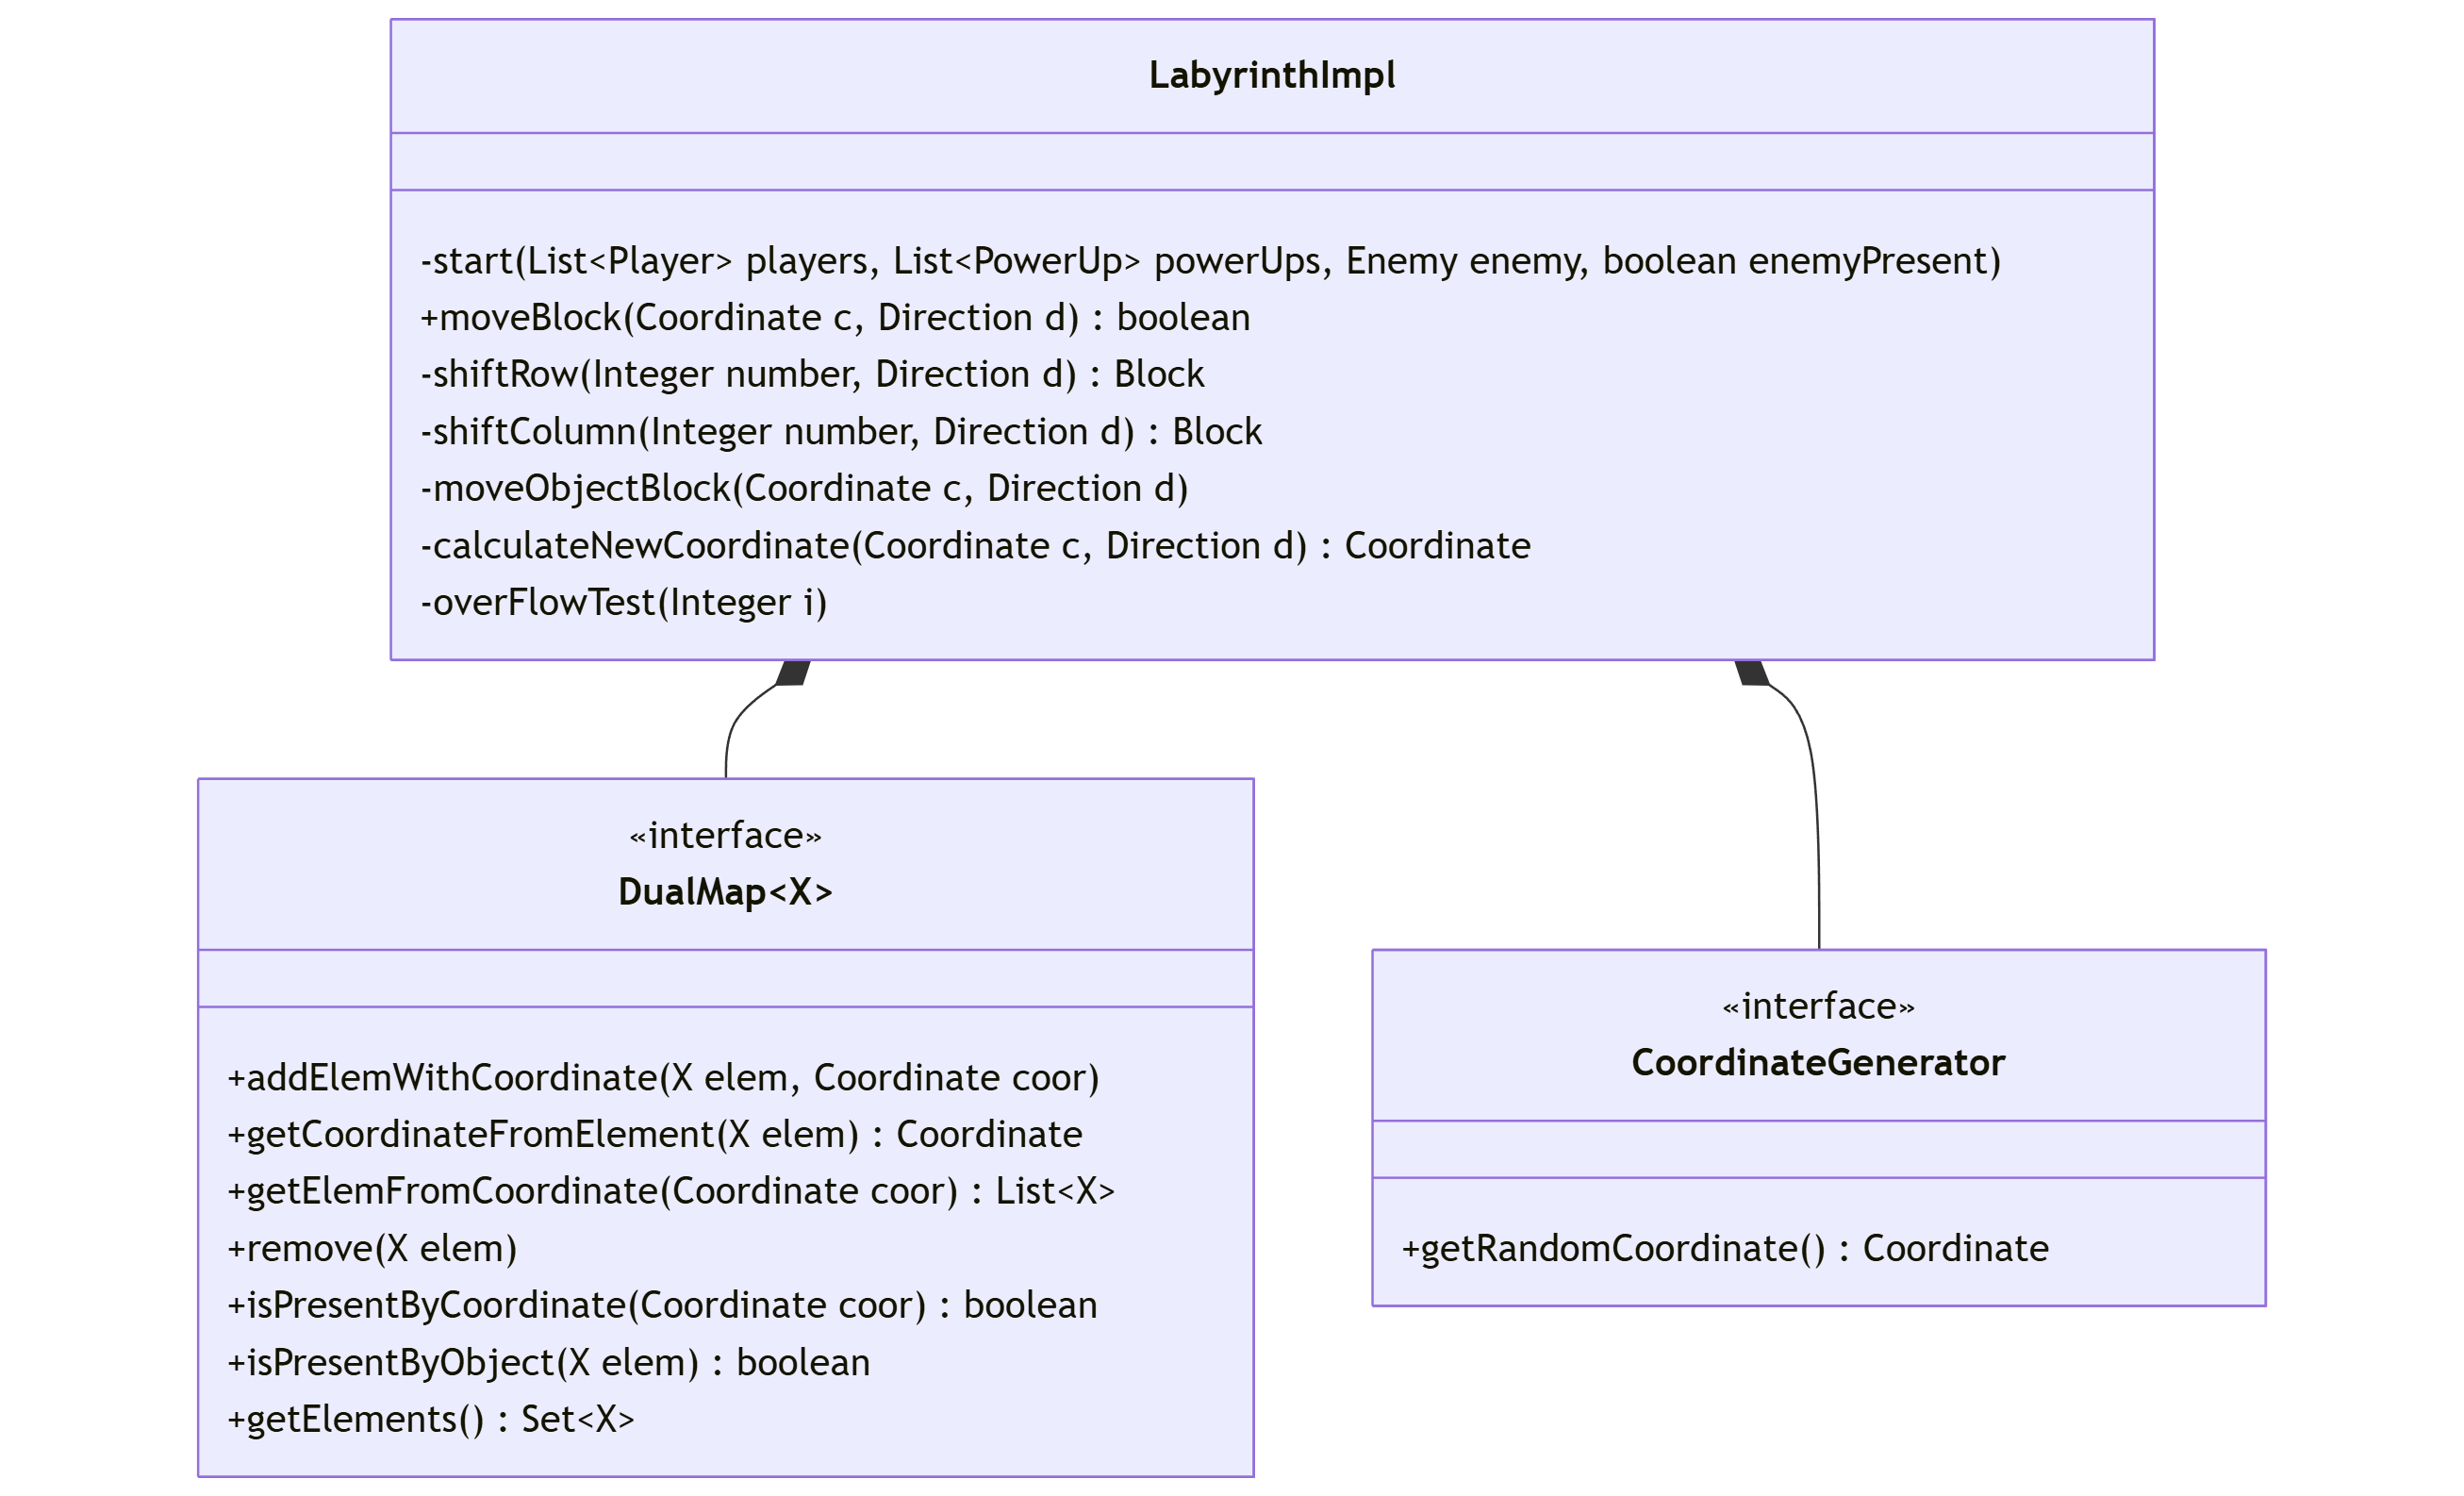
\includegraphics[width=14cm]{img/GestioneCoordinate.png}
	\caption{Schema UML del processo per la gestione delle coordinate}
	\label{img:Gestione Coordinate}
\end{figure}
\textbf{Caricamento immagini e disegno grafica}
\\
\\
\textbf{PROBLEMA}
Nel contesto del gioco ispirato al Labirinto Magico, è essenziale offrire all’utente una rappresentazione grafica chiara, coerente e reattiva dello stato di gioco. 
La visualizzazione deve adattarsi dinamicamente alle dimensioni della finestra e 
riflettere fedelmente ogni modifica del modello, inclusi la rotazione delle tessere, la posizione dei giocatori, la presenza di obiettivi o nemici.
\\
\\
\textbf{SOLUZIONE}
Per affrontare questo problema ho adottato una chiara separazione tra la logica di visualizzazione e rendering grafico.
In particolare la soluzione che ho adottato utilizza 3 componenti.
\begin{itemize}
	\item \textbf{DrawPanel}: componente di basso livello incaricato esclusivamente del disegno su schermo. Riceve una lista strutturata di elementi grafici già processati e li renderizza.
	\item \textbf{LogicDrawPanel}: componente intermedio creato dal DrawPanel che si occupa della logica di visualizzazione. 
	Analizza lo stato del modello (GameController), calcola le coordinate pixel, la rotazione e la dimensione ottimale per ogni immagine da disegnare.
	\item \textbf{ImageLoader}:  classe dedicata al caricamento e alla gestione delle risorse grafiche. Associa ogni elemento di gioco alla sua rispettiva immagine.
\end{itemize}
Quando la GameView richiede un aggiornamento:
\begin{itemize}
	\item Il DrawPanel interroga il LogicDrawPanel.
	\item Il LogicDrawPanel analizza lo stato corrente del gioco e costruisce più elementi contenenti tutte le informazioni utili per il rendering.
	\item Il DrawPanel renderizza tale rappresentazione.
\end{itemize}
Il calcolo delle proporzioni avviene dinamicamente in base alla dimensione della finestra dell’applicazione, garantendo un’interfaccia responsive. 
In fondo a tutto ciò ho anche deciso di aggiungere per ogni giocatore un'immagine uguale al suo personaggio ma cambiata di colore per indicare graficamente, 
il giocatore che sta svolgendo il turno.
\\
\\
\textbf{PRO}
\begin{itemize}
	\item La separazione tra logica e rendering consente una maggiore manutenibilità e una lettura più chiara del codice.
	\item L'interfaccia utente si adatta automaticamente alla risoluzione della finestra.
	\item Si possono aggiungere facilmente nuove funzionalità grafica o set di elementi senza dover apportare modifiche al codice già implementato.
\end{itemize}
\textbf{CONTRO}
\begin{itemize}
	\item In caso di aggiornamento del model il LogicDrawPanel si deve ricalcolare tutti gli elementi anche quelli non modificati di posizione o rotazione.
\end{itemize}
\begin{figure}[H]
	\centering{}
	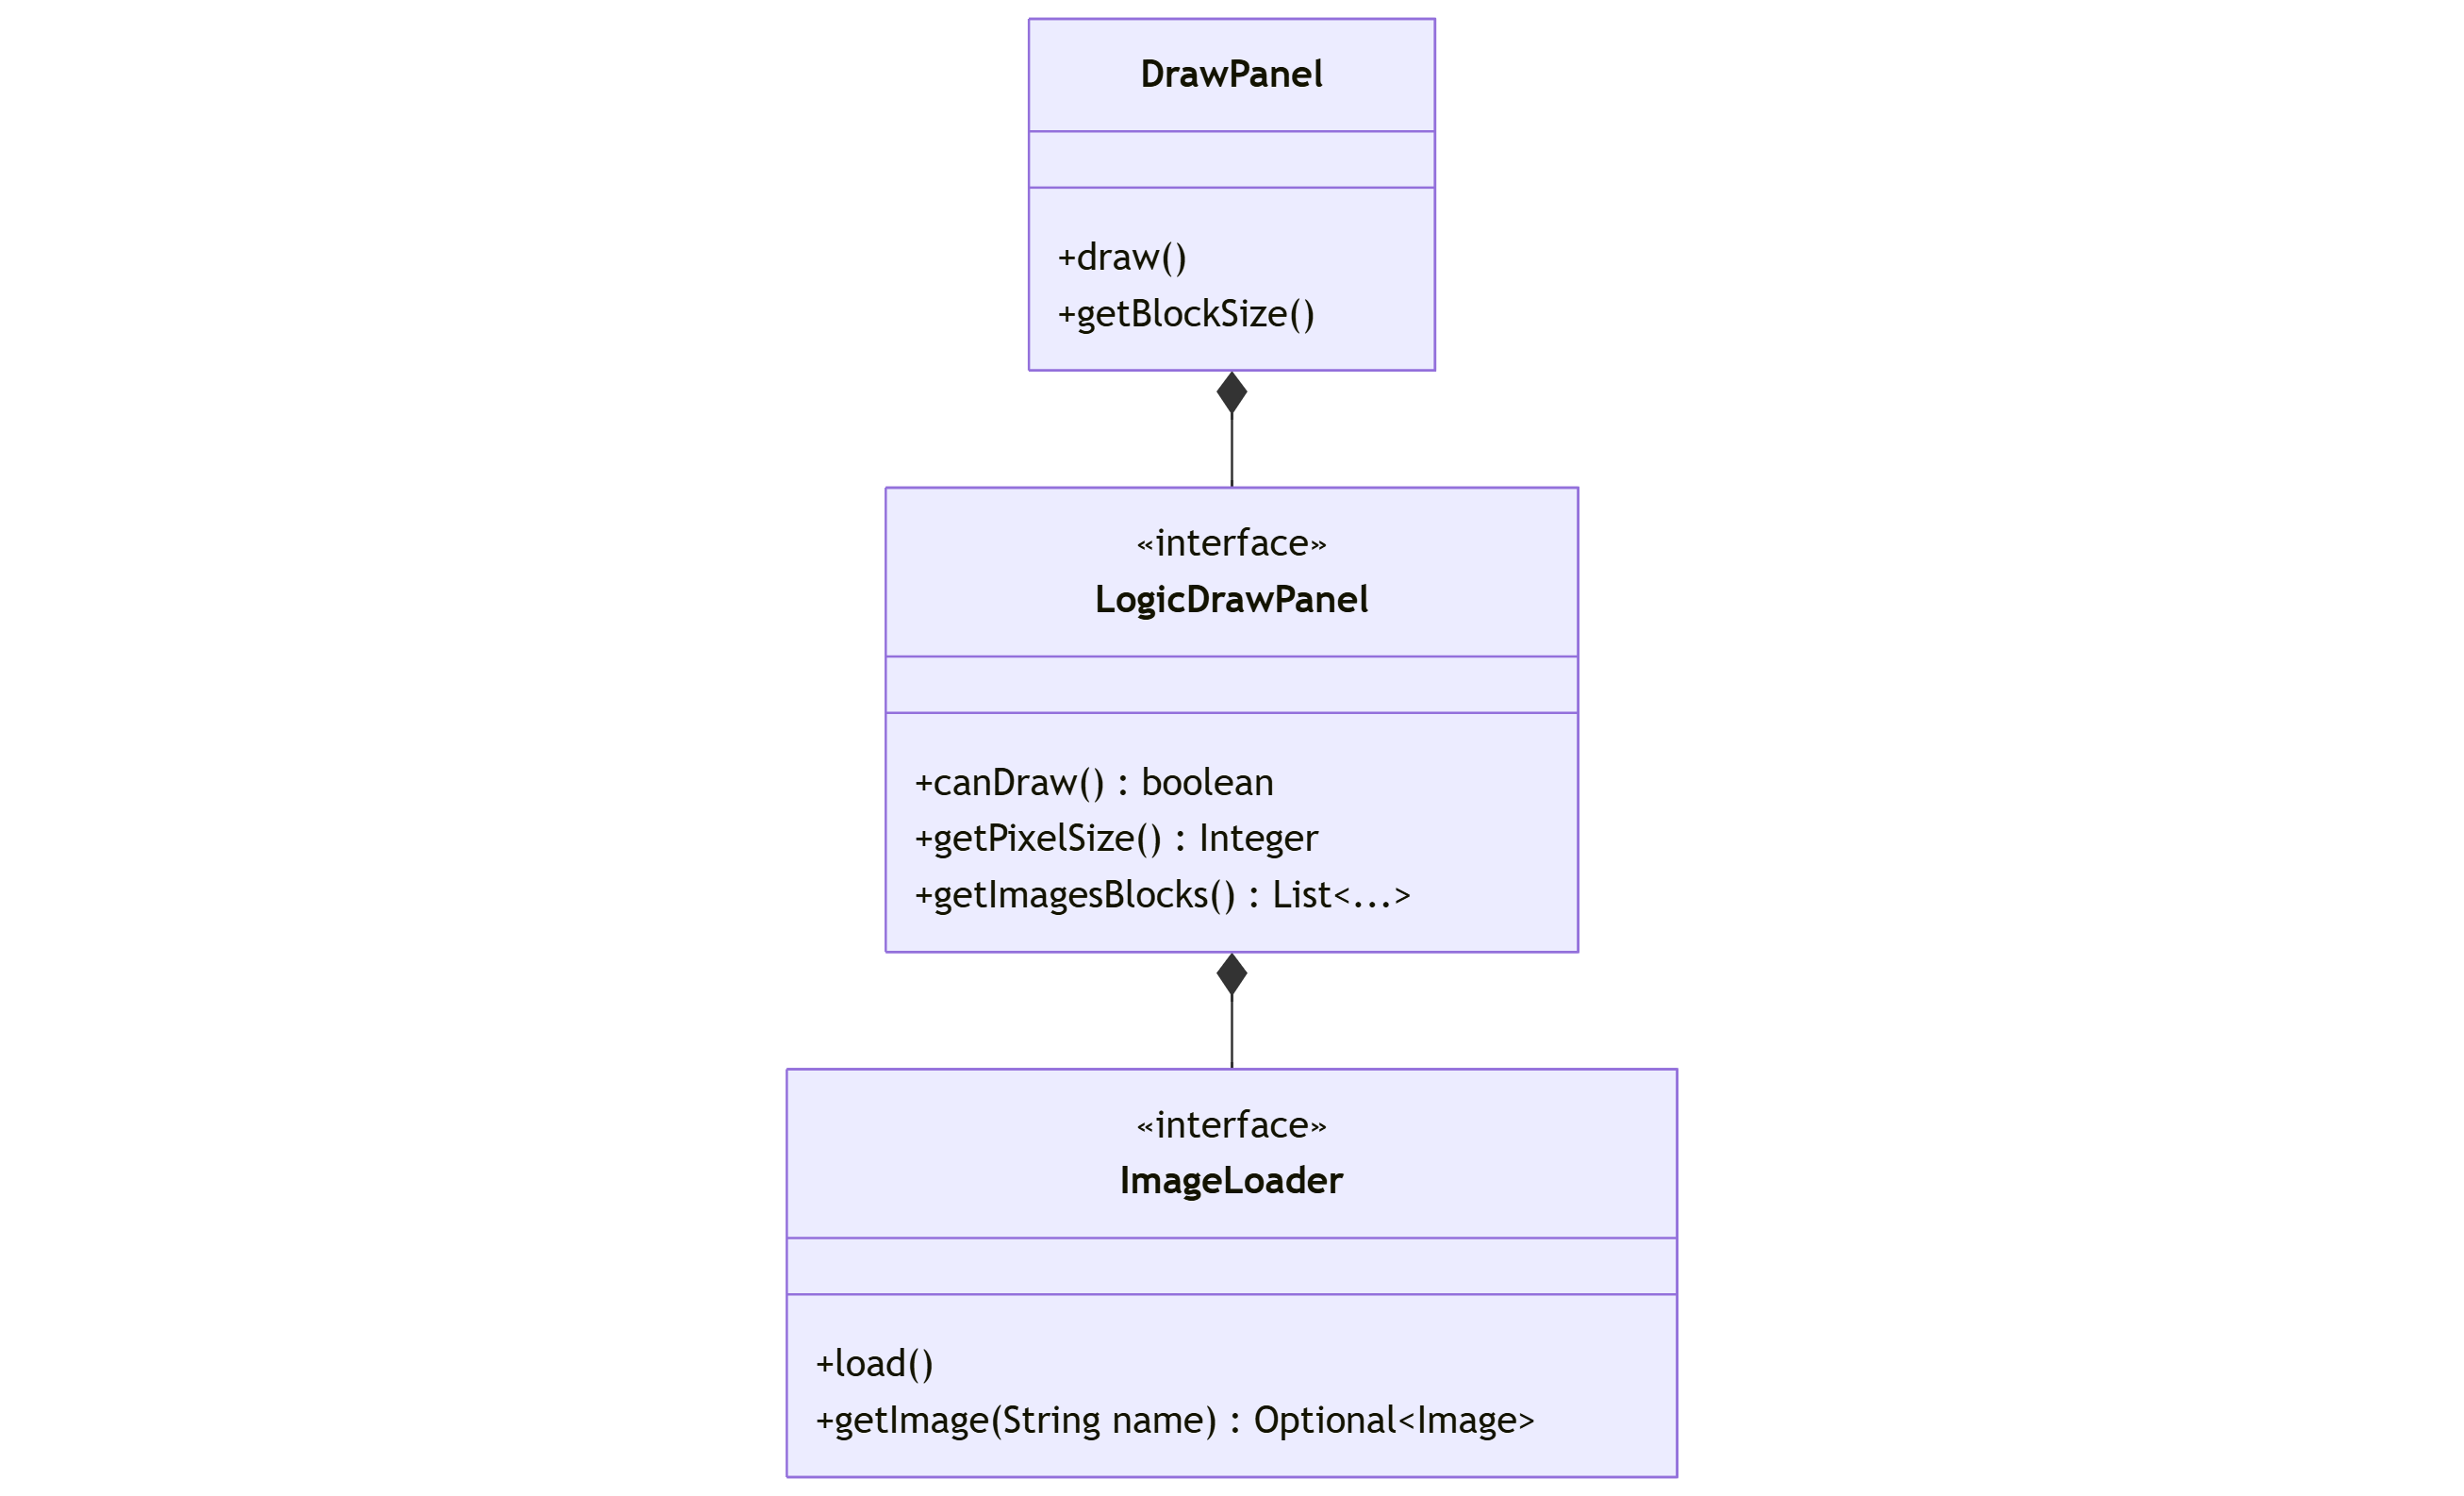
\includegraphics[width=14cm]{img/DisegnareGrafica.png}
	\caption{Schema UML del processo per aggiornare la grafica di gioco}
	\label{img:Aggiornamento Grafica}
\end{figure}
\textbf{Metodi per la gestione dei punteggi, nomi e informazioni}
\\
\\
\textbf{PROBLEMA}
Durante lo svolgimento della partita, è fondamentale fornire al giocatore un feedback continuo sullo stato del gioco. In particolare, è necessario visualizzare:
\begin{itemize}
	\item A chi tocca il turno corrente.
	\item Qual è l’azione richiesta.
	\item I power-up utilizzabili per ciascun giocatore.
	\item Il vincitore della partita (quando rilevante).
	\item Una classifica aggiornata dei giocatori con informazioni sul punteggio e lo stato.
\end{itemize}
Queste informazioni devono essere rese accessibili in modo intuitivo e integrato nell’interfaccia utente, 
senza legare la logica della visualizzazione direttamente al modello del gioco.
\\
\\
\textbf{SOLUZIONE}
Per separare correttamente la logica del gioco dalla logica di presentazione, è stata introdotta una componente intermedia: la \textbf{LogicGameView}.
In questa classe io ho creato delle funzionalità per la trasformazione di informazioni dal model in stringe comprensibili dall'utente e mostrabili dalla view.
Tra queste ci sono:
\begin{itemize}
	\item Turni e azioni: restituisce il nome del giocatore a cui tocca e la descrizione dell’azione da compiere.
	\item Power-Up: crea e restituisce una lista dei power-up attivi utilizzabili da un giocatore, da mostrare tramite ComboBox.
	\item Esito della partita: genera un messaggio da visualizzare alla fine del gioco, indicando il vincitore.
	\item Classifica giocatori: restituisce, per ciascun giocatore, una stringa contenente nome, punteggio e stato.
\end{itemize}
\textbf{PRO}
\begin{itemize}
	\item Separazione delle responsabilità: La logica trasforma i dati e li passa alla view rendendosi intermediaria tra l'interfaccia utente e il model.
	\item Manutenibilità: In caso di future modifiche alla stringhe da visualizzare si possono cambiare codici poco complessi e distaccati dalla view quindi di facile elaborazione.
	\item Flessibilità: in caso di necessità queste informazioni possono essere mostrate dalla view in modi differenti senza dover ricorrere a un ricalcolo delle stringhe.
\end{itemize}
\textbf{CONTRO}
\begin{itemize}
	\item Bisogna dare paricolare attenzione agli aggiornamenti della view perché in caso di cambiamento del model ma non della view si prensenta per l'utente della confusione 
	nello stato della partita.
\end{itemize}
\begin{figure}[H]
	\centering{}
	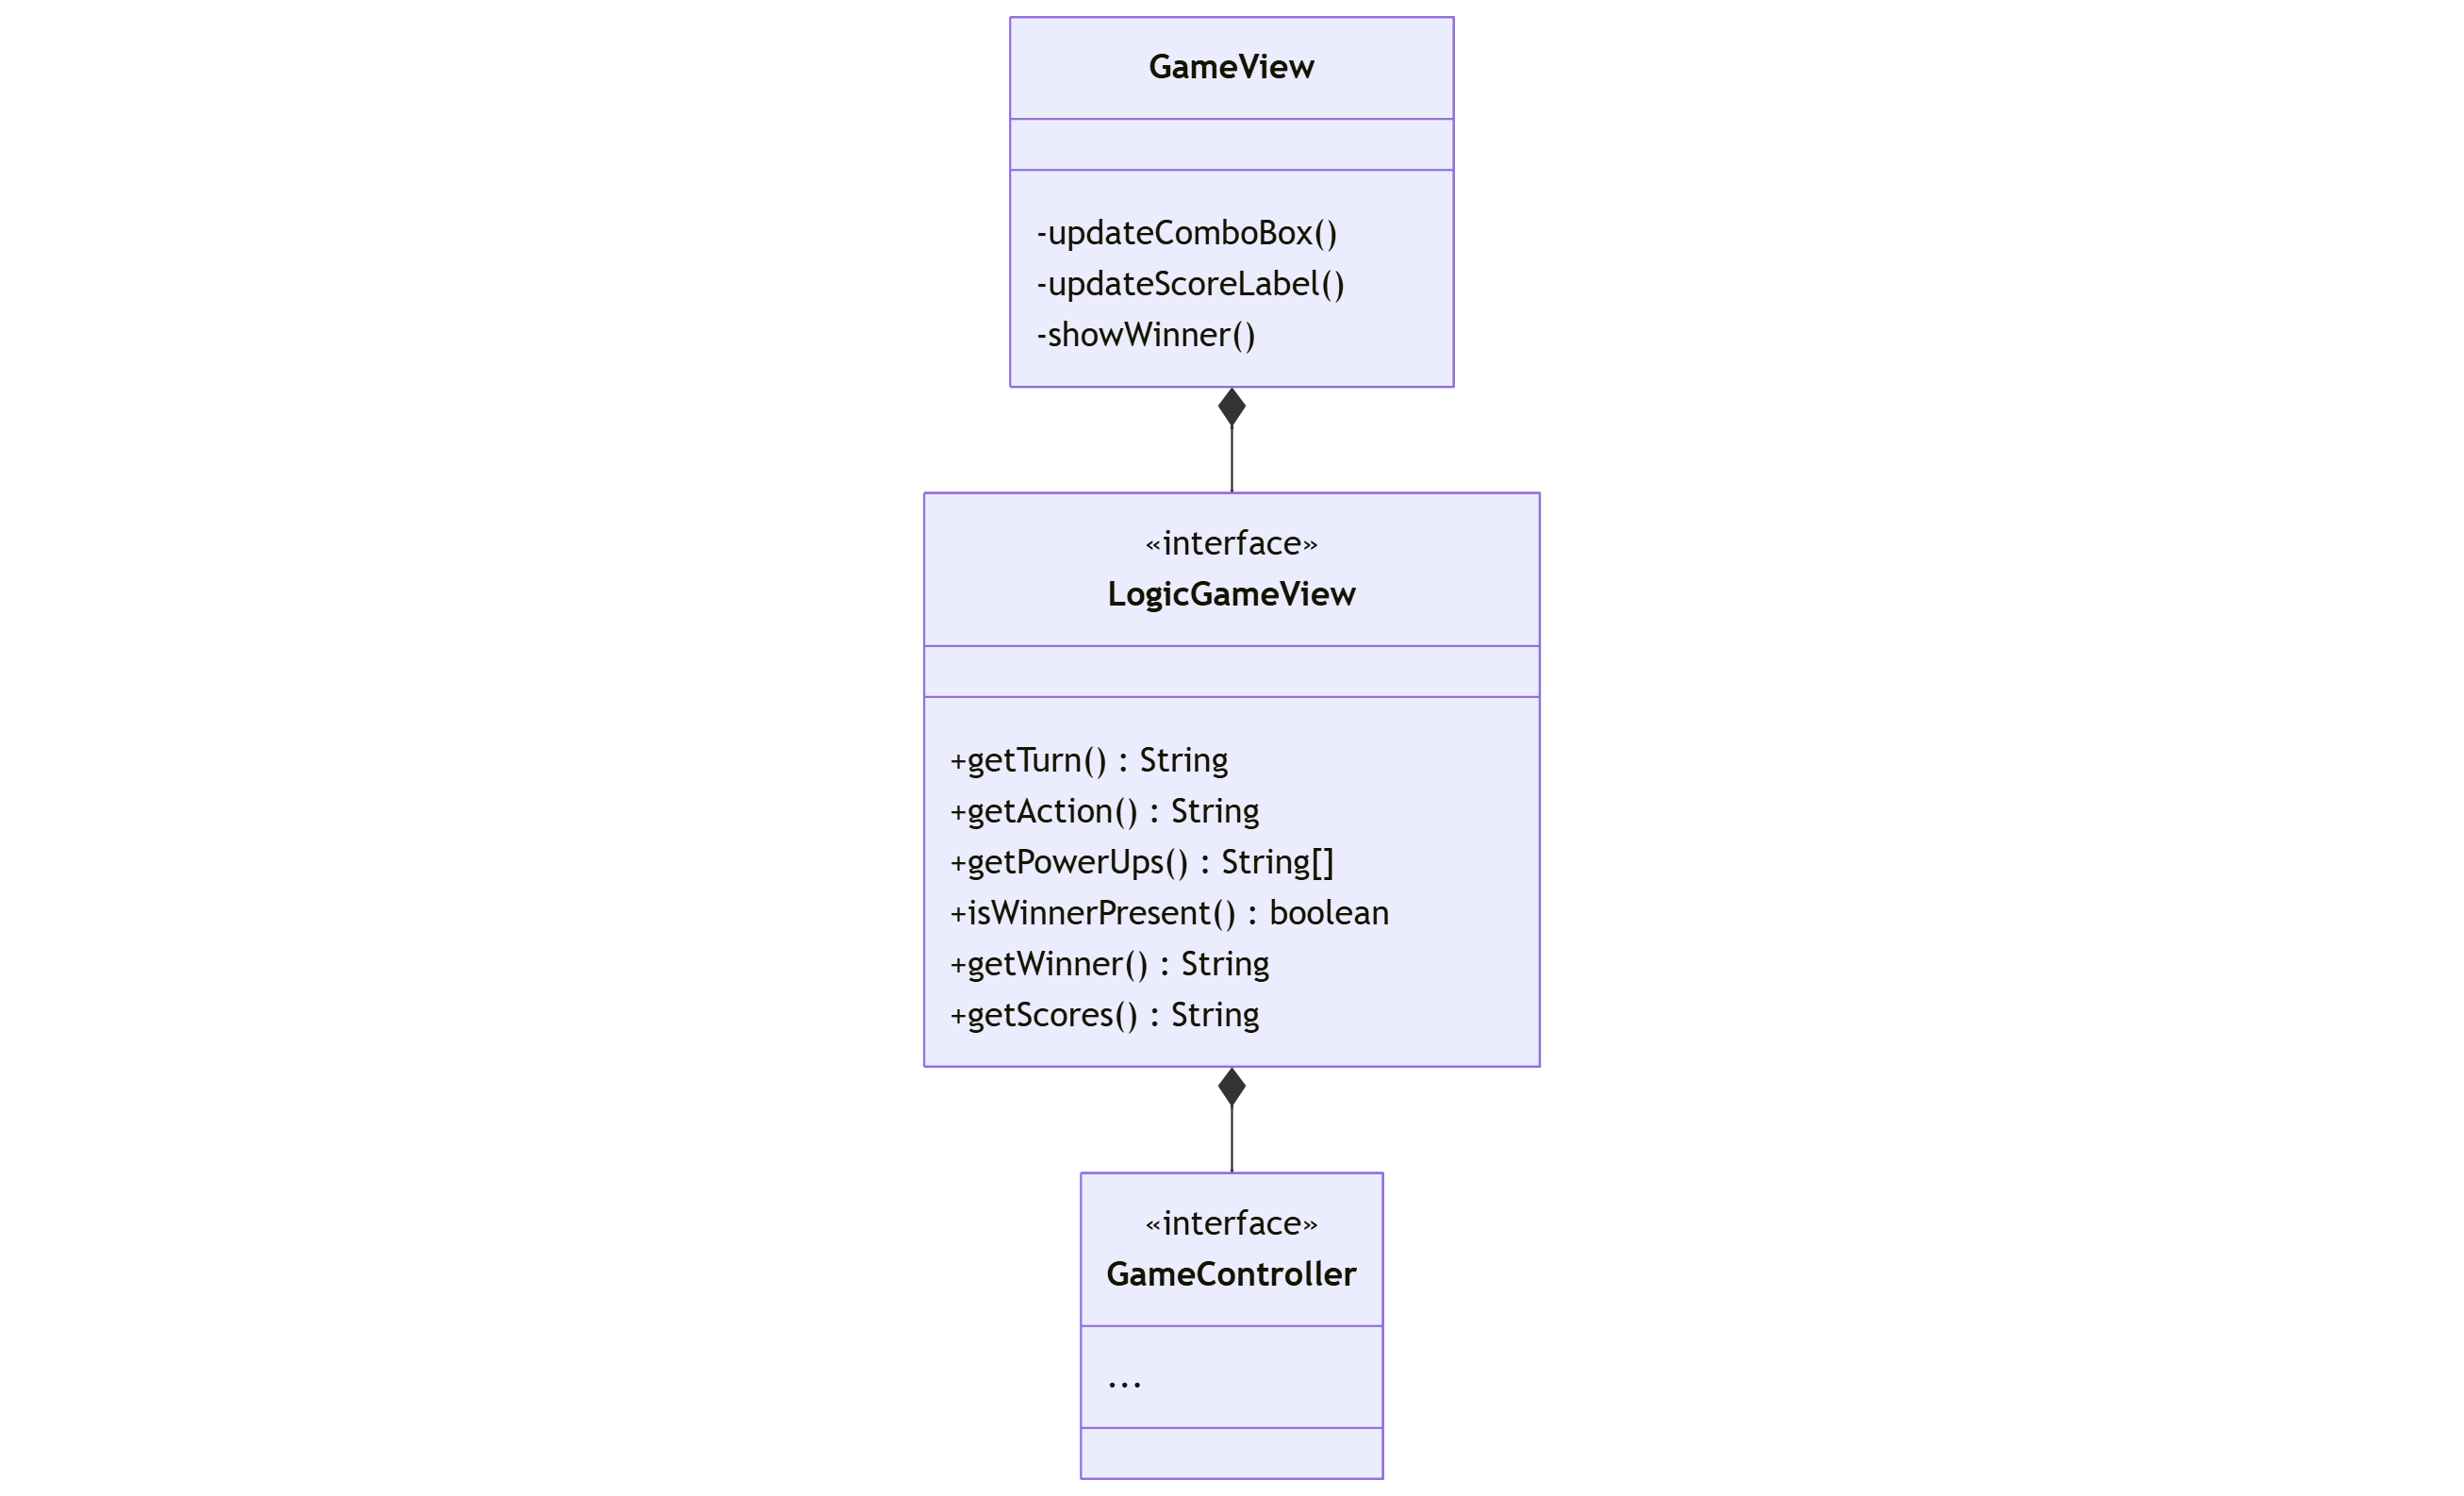
\includegraphics[width=14cm]{img/TraduzioneInformazioni.png}
	\caption{Schema UML dei processi per leggere le informazioni dal gioco}
	\label{img:Traduzione Informazioni}
\end{figure}

\chapter{Sviluppo}
\section{Testing automatizzato}

Per verificare il corretto funzionamento delle diverse parti del progetto, sono
 stati creati Test automatizzati usando JUnit.

\subsection{Enrico Ancarani}
\begin{itemize}
	\item \textbf{BlockTest}: verifica la corretta creazione delle tessere e il funzionamento della rotazione. I test accertano che, a seguito della rotazione, 
	l’orientamento della tessera cambi come previsto.
	\item \textbf{GenerateMazeTest}: verifica la correttezza della generazione iniziale della mappa di gioco. In particolare, si controlla che:
	\begin{itemize}
		\item tutte le tessere abbiano coordinate valide all’interno del labirinto.
		\item non vi siano duplicati (ovvero, che ogni tessera sia presente in una sola posizione).
		\item il blocco esterno venga generato correttamente.
		\item i blocchi iniziali dei giocatori siano posizionati correttamente.
	\end{itemize}
	\item \textbf{PositioningTest}: controlla che ogni elemento abbia una posizione nel labirinto e che i giocatori siano inizilizzati nelle giuste posizioni.
	Poi controlla che se effettuata una modifica alla posizione di un elemento essa non presenta errori e viene salvata correttamente.
	\item \textbf{ShiftsTest}: verifica il comportamento dello shift del labirinto. Dopo l’esecuzione dello spostamento, si controlla che 
	tutte le tessere siano state aggiornate nella posizione corretta e che il blocco esterno sia stato gestito coerentemente.
	\item \textbf{PlayerTest}: verifica il corretto comportamento del player nelle situazioni:
	\begin{itemize}
		\item raccolta di un obbietivo.
		\item utilizzo di un powerUp.
		\item movimento.
	\end{itemize}
\end{itemize}

\section{Note di sviluppo}

\subsection{Enrico Ancarani}
\begin{itemize}
	\item \textbf{Utilizzo di Optional}: Utilizzato in vari punti, un esempio è: \url{https://github.com/EnricoAncaraniUnibo/OOP24-LabiOOPint/blob/bff4699198b12c8ac5b1b91a798ec85b5443a107/src/main/java/labioopint/model/maze/impl/MazeImpl.java#L46}
	\item \textbf{Utilizzo di Stream}: Utilizzato in vari punti, un esempio è: \url{https://github.com/EnricoAncaraniUnibo/OOP24-LabiOOPint/blob/bff4699198b12c8ac5b1b91a798ec85b5443a107/src/main/java/labioopint/model/maze/impl/LabyrinthImpl.java#L355}
	\item \textbf{Utilizzo di Lambda expressions}: Utilizzato nella classe LabyrinthImpl: \url{https://github.com/EnricoAncaraniUnibo/OOP24-LabiOOPint/blob/bff4699198b12c8ac5b1b91a798ec85b5443a107/src/main/java/labioopint/model/maze/impl/LabyrinthImpl.java#L386}
\end{itemize}

\chapter{Commenti finali}

In quest'ultimo capitolo si tirano le somme del lavoro svolto e si delineano eventuali sviluppi
futuri.

\textit{Nessuna delle informazioni incluse in questo capitolo verrà utilizzata per formulare la valutazione finale}, a meno che non sia assente o manchino delle sezioni obbligatorie.
%
Al fine di evitare pregiudizi involontari, l'intero capitolo verrà letto dai docenti solo dopo aver formulato la valutazione.

\section{Autovalutazione e lavori futuri}

\subsection{Enrico Ancarani}
Questa non rappresentava la mia prima esperienza di lavoro in team per lo sviluppo di un progetto software complesso. 
Per questo motivo, ritengo che la mia presenza all'interno del gruppo sia stata un supporto utile anche per gli altri membri, sia dal punto di vista tecnico che organizzativo.
Il mio ruolo si è concentrato principalmente sulla modellazione della mappa di gioco, sulla gestione delle coordinate e degli elementi associati alla mappa, 
sull’aggiornamento grafico delle immagini e sulla gestione della logica relativa ai giocatori. Ho partecipato attivamente a ogni fase del progetto, mettendo impegno 
costante durante gli incontri e lavorando in modo continuativo tra una sessione e l’altra.
Tra i miei punti di forza riconosco la determinazione nel portare a termine le attività assegnate senza rimandare, la capacità di spiegare con chiarezza aspetti 
implementativi complessi agli altri membri del gruppo, e l'iniziativa nel proporre soluzioni rapide ed efficaci ai problemi riscontrati durante la scrittura del codice. 
Inoltre, ho cercato di mantenere alta la motivazione del team nei momenti di difficoltà.
D’altra parte, tra i miei punti di debolezza evidenzio una certa testardaggine nel difendere le mie proposte e la tendenza ad assumere un ruolo di leadership anche 
quando non esplicitamente richiesto, specialmente durante la fase di progettazione dell’architettura.
Le principali difficoltà riscontrate hanno riguardato l’utilizzo efficace di GitHub per il lavoro collaborativo e l’applicazione corretta e coerente del pattern 
architetturale MVC, soprattutto nelle prime fasi di sviluppo.
In conclusione, considero il mio contributo positivo e sono soddisfatto dell’impegno personale e del risultato ottenuto. 
Se in futuro si decidesse di proseguire con lo sviluppo del progetto, si potrebbe arricchire il gioco introducendo nuovi obiettivi, 
power-up, scenari alternativi con tessere speciali o strutture della mappa più articolate, al fine di aumentare la varietà e la profondità dell’esperienza di gioco.
\\
\\
\appendix
\chapter{Guida utente}

Capitolo in cui si spiega come utilizzare il software. Nel caso in cui il suo uso sia del tutto
banale, tale capitolo può essere omesso.
%
A tal riguardo, si fa presente agli studenti che i docenti non hanno mai utilizzato il software
prima, per cui aspetti che sembrano del tutto banali a chi ha sviluppato l'applicazione possono non
esserlo per chi la usa per la prima volta.
%
Se, ad esempio, per cominciare una partita con un videogioco è necessario premere la barra
spaziatrice, o il tasto ``P'', è necessario che gli studenti lo segnalino.

\subsection*{Elementi positivi}

\begin{itemize}
 \item Si istruisce in modo semplice l'utente sull'uso dell'applicazione, eventualmente facendo uso di schermate e descrizioni.
\end{itemize}

\subsection*{Elementi negativi}
\begin{itemize}
 \item Si descrivono in modo eccessivamente minuzioso tutte le caratteristiche, anche minori, del software in oggetto.
 \item Manca una descrizione che consenta ad un utente qualunque di utilizzare almeno le funzionalità primarie dell'applicativo.
\end{itemize}

\chapter{Esercitazioni di laboratorio}

In questo capitolo ciascuno studente elenca gli esercizi di laboratorio che ha svolto
(se ne ha svolti),
elencando i permalink dei post sul forum dove è avvenuta la consegna.
%
Questa sezione potrebbe essere processata da strumenti automatici,
per cui link a oggetti diversi dal permalink della consegna,
errori nell'email o nel nome del laboratorio possono portare ad ignorare alcune consegne,
si raccomanda la massima precisione.

\section*{Esempio}

\subsection{paolino.paperino@studio.unibo.it}

\begin{itemize}
 \item Laboratorio 04: \url{https://virtuale.unibo.it/mod/forum/discuss.php?d=12345#p123456}
 \item Laboratorio 06: \url{https://virtuale.unibo.it/mod/forum/discuss.php?d=22222#p222222}
 \item Laboratorio 09: \url{https://virtuale.unibo.it/mod/forum/discuss.php?d=99999#p999999}
\end{itemize}

\subsection{paperon.depaperoni@studio.unibo.it}

\begin{itemize}
 \item Laboratorio 04: \url{https://virtuale.unibo.it/mod/forum/discuss.php?d=12345#p123456}
 \item Laboratorio 05: \url{https://virtuale.unibo.it/mod/forum/discuss.php?d=22222#p222222}
 \item Laboratorio 06: \url{https://virtuale.unibo.it/mod/forum/discuss.php?d=99999#p999999}
 \item Laboratorio 07: \url{https://virtuale.unibo.it/mod/forum/discuss.php?d=22222#p222222}
 \item Laboratorio 08: \url{https://virtuale.unibo.it/mod/forum/discuss.php?d=99999#p999999}
 \item Laboratorio 09: \url{https://virtuale.unibo.it/mod/forum/discuss.php?d=22222#p222222}
 \item Laboratorio 10: \url{https://virtuale.unibo.it/mod/forum/discuss.php?d=99999#p999999}
 \item Laboratorio 11: \url{https://virtuale.unibo.it/mod/forum/discuss.php?d=22222#p222222}
\end{itemize}

\end{document}
